\section{Анализ предметной области}
\label{sec:analysis}

Извлечение музыкальной информации - небольшая, но интересная и быстрорастущая область исследований, которая охватывает большой диапазон продуктов, используемых по всему миру. Эта область охватывает \linebreak несколько дисциплин научных знаний: музыковедение, психологию, обработку сигналов, машинное обучение и комбинации этих дисциплин. Задача, которую будет решать разрабатываемый сервис, относится к задачам извлечения музыкальной информации.

Несмотря на то, что извлечение музыкальной информации является еще небольшой областью исследований, для извлечения характеристик музыкальных приложений применяется достаточное количество методов. Эти методы различаются как на основаниии применяемых подходов, так и на основании уровней извлекаемых характеристик. На основании характеристик выделяют методы, которые извлекают низкоуровневые характеристики (спектр, ритм), и методы которые извлекают высокоуровневые характеристики (жанр, настроение). В основном, нас будут интересовать методы, которые извлекают высокоуровневые характеристики.

Для извлечения высокоуровневых характеристик выделяют два класса методов: основанные на математических функциях, в основе которых лежит машинное обучение. В музыке появляются новые направления, а старые могут изменяться, поэтому наиболее перспективными являются методы, которые способны постраиваться под переменчивую природу музыки. Под такие условия в большей степени подходят методы, в основе которых лежит машинное обучение.

Машинное обучение - класс методов, характерной чертой которых является не прямое решение задачи, а решение, которое строится в процессе обучения при применении решения к множеству сходных задач. В последнее время этот класс методов получил активное развитие и поддержку со стороны крупных компаний и университетов.

Цифровой аудиосигнал можно представить в виде изображения звуковой волны (см. рисунок \ref{sec:analysus:sound_wave}).

\begin{figure}[t]
\centering
	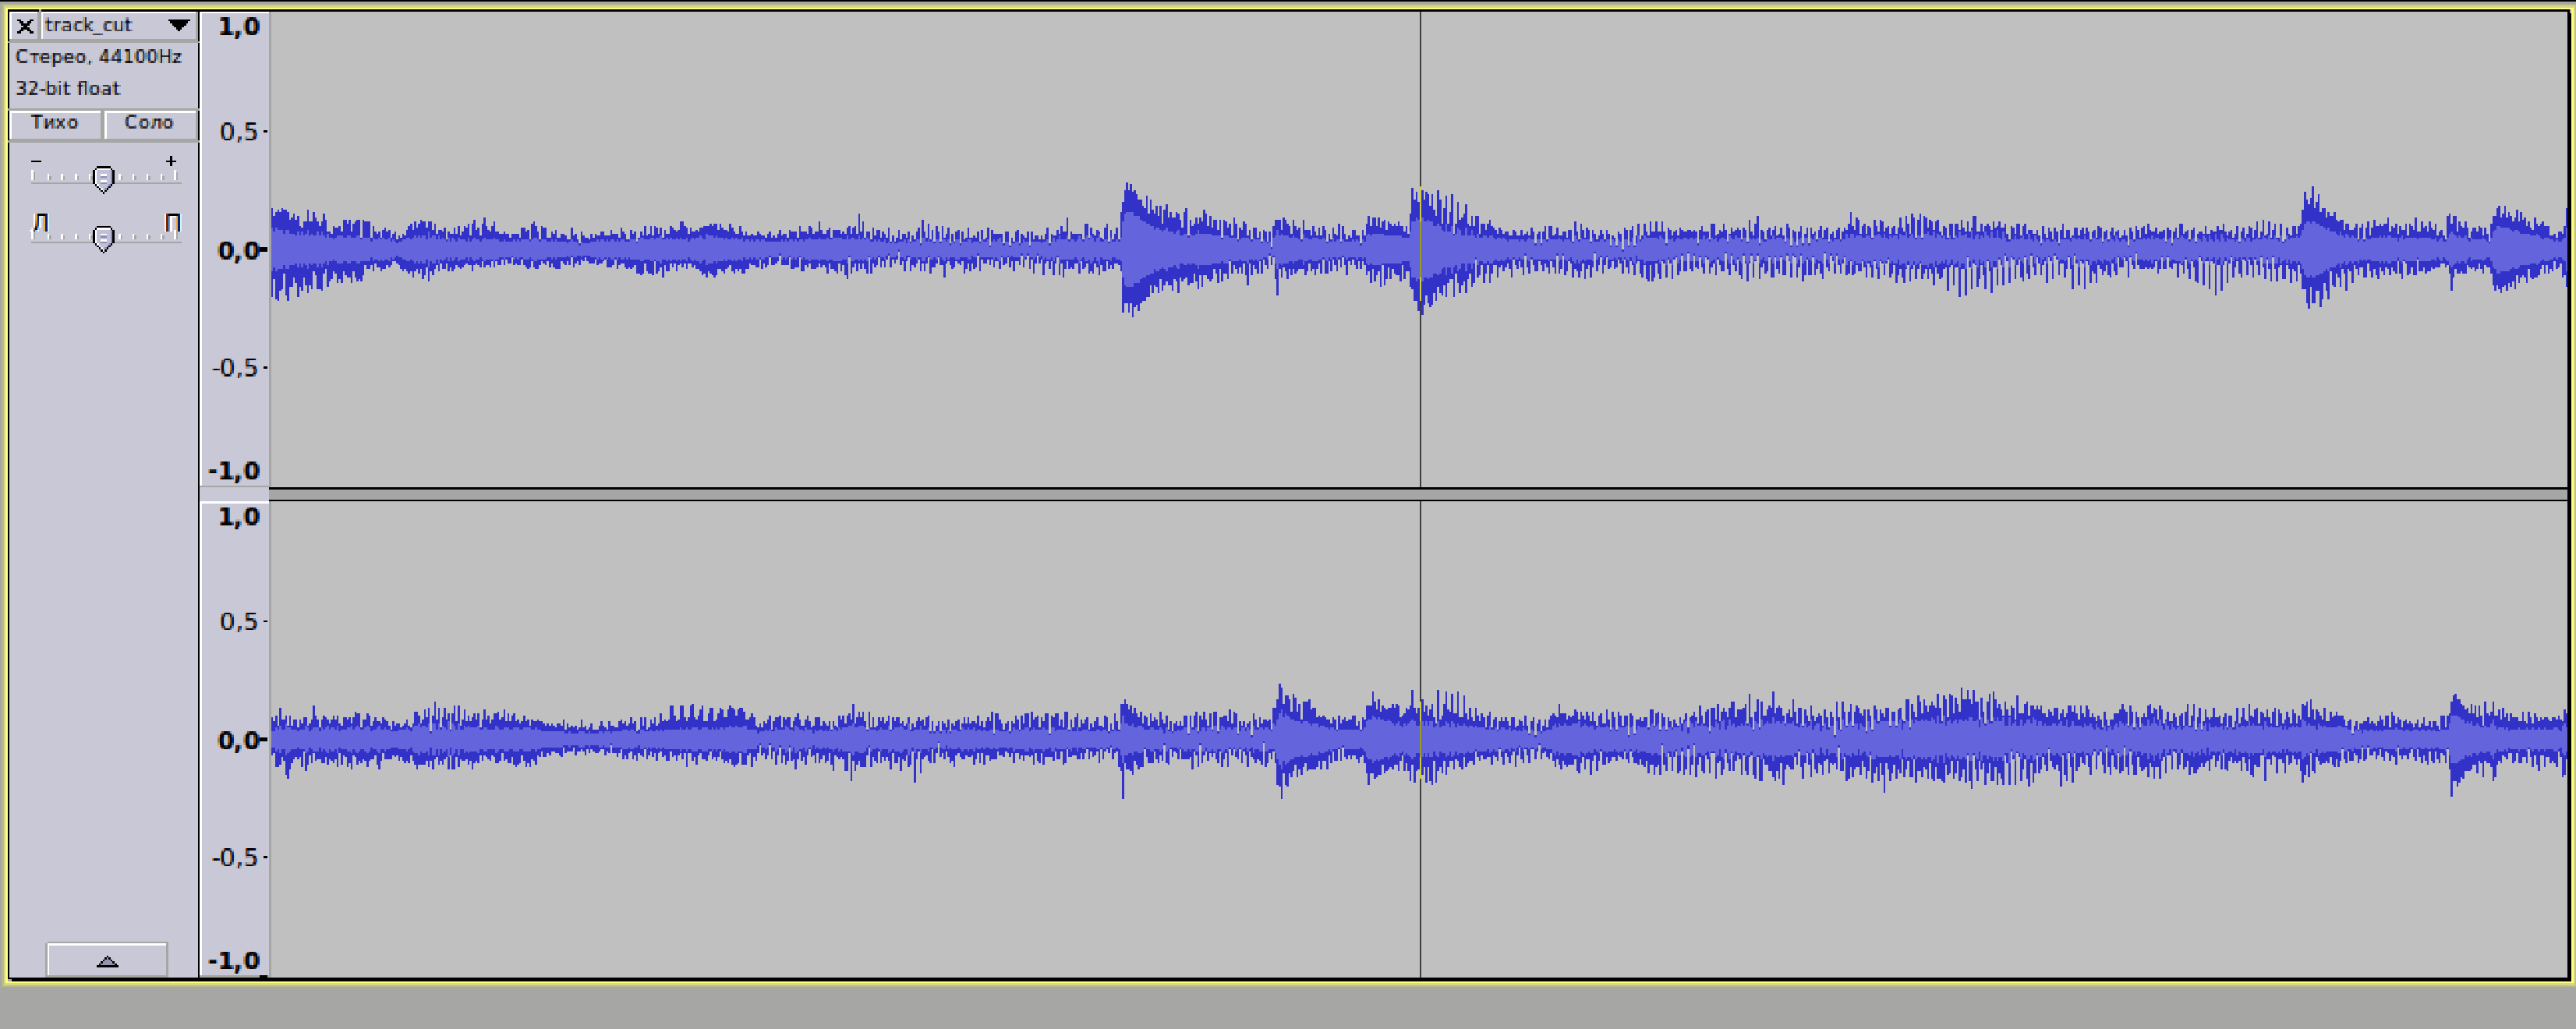
\includegraphics[scale=0.14]{attachments/sound_vawe.png}
	\caption{Изображение звуковой волны}
	\label{sec:analysus:sound_wave}
\end{figure}

Цифровой аудиосигнал представляет собой множество точек, которые расставлены на одинаковом расстоянии друг от друга (см. рисунок \ref{sec:analysus:sound_wave_hi}). Расстояние между точками называется частотой дискретизации. Чем меньше интервал (выше частота дискретизации), тем шире частотный диапазон, который можно закодировать таким образом.

\begin{figure}[t]
\centering
	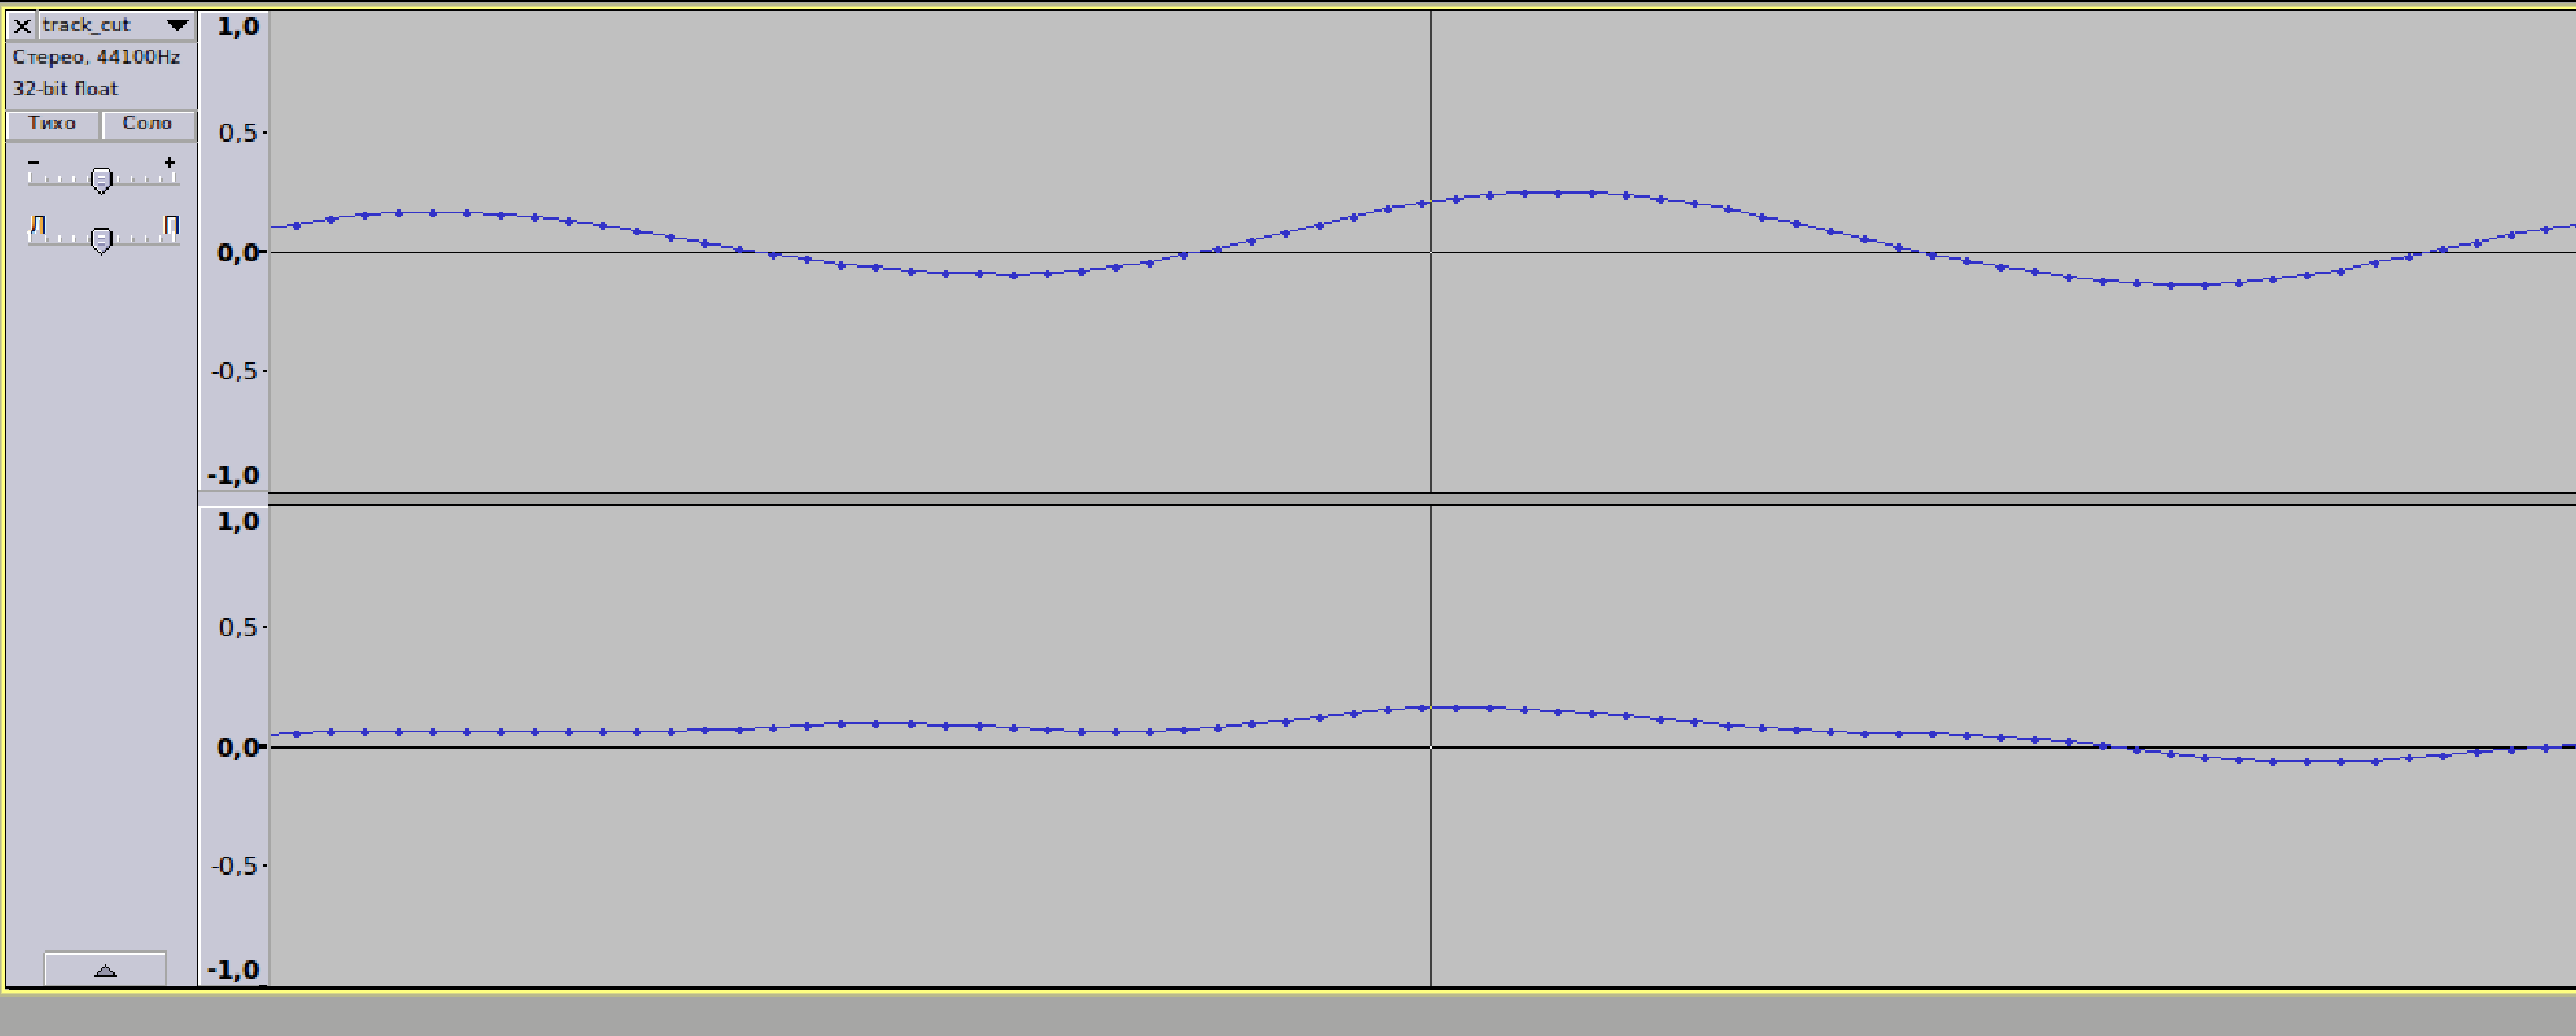
\includegraphics[scale=0.14]{sound_wave_hi.png}
	\caption{Изображение звуковой волны в большом разрешении}
	\label{sec:analysus:sound_wave_hi}
\end{figure}

Амплитуда колебаний зависит от времени звука и коррелирует с громкостью звука. А частота колебаний напрямую связана с высотой звука. Для того, чтобы получить информацию о частоте колебаний, необходимо применить преобразование Фурье. Преобразование Фурье позволяет разложить периодическую функцию в сумму гармонических с разными частотами. Коэффициенты гармонических функций при сложении будут давать нам те частоты, которые мы хотим получить.

При применении преобразования Фурье ко всей звуковой дорожке мы получим "смазанный" во времени спектр. Для того, чтобы получить спектр, не теряя временной составляющей, необходимо применить к сигналу оконное преобразование Фурье. Оконное преобразование Фурье отличается от обычного тем, что мы делим наш сигнал на короткие отрезки (окна) и применяем к каждому преобразование Фурье. По-сути мы получаем набор спектров: отдельно для каждого отрезка. В результате мы получим картинку, которой можно описать звуковую дорожку (см. рисунок \ref{sec:analysus:spectrum}).

\begin{figure}[h]
\centering
	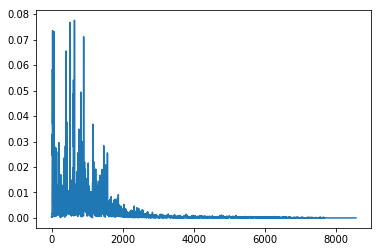
\includegraphics[scale=1.2]{spectrum.png}
	\caption{Спектральная характеристика}
	\label{sec:analysus:spectrum}
\end{figure}

Жанр композиции является высокоуровневой характеристикой. Для определения жанра необходимо разобраться, как человек воспринимает звук.

Ухо человека устроено так: звуковые волны смещают барабанную перепонку при взаимодействии с ней. Вибрации передаются во внутреннее ухо и считываются им. Смещение барабанной перепонки зависит от звукового давления, при том зависимость является не линейной, а логарифмической. Для измерения громкости принято использовать относительную шкалу - уровень звукового давления (измеряется в децибелах). Так же воспринимаемая громкость зависит и от частоты звука. Для оценки громкости звука используется логарифмическая единица измерения - фон. В шкале фонов, в отличие от децибелов, значения громкости связаны с чувствительностью на разных частотах человеческого уха. Частота 1000 Гц является чистым тоном, и уровень фона для неё численно равен уровню в децибелах. Для остальных частот используют поправки, которые представляют собой стандартизированное семейство кривых, называемых изофонами (см. рисунок \ref{sec:analysus:sound_contur}).

Аналогично с громкостью, частота так же воспринимается человеческим ухом нелинейно. Для измерения воспринимаемой частоты человеческим ухом используется мел-шкала (см. рисунок \ref{sec:analysus:mel}). Шкала основана на статистической обработке субъективного восприятия звука на больших данных. За 1000 мел взят звук с частотой 1000 Гц при уровне громкости 40 фон. За 0 мел взят звук частотой 20 Гц при уровне громкости 40 фон.

\begin{figure}[h]
\centering
	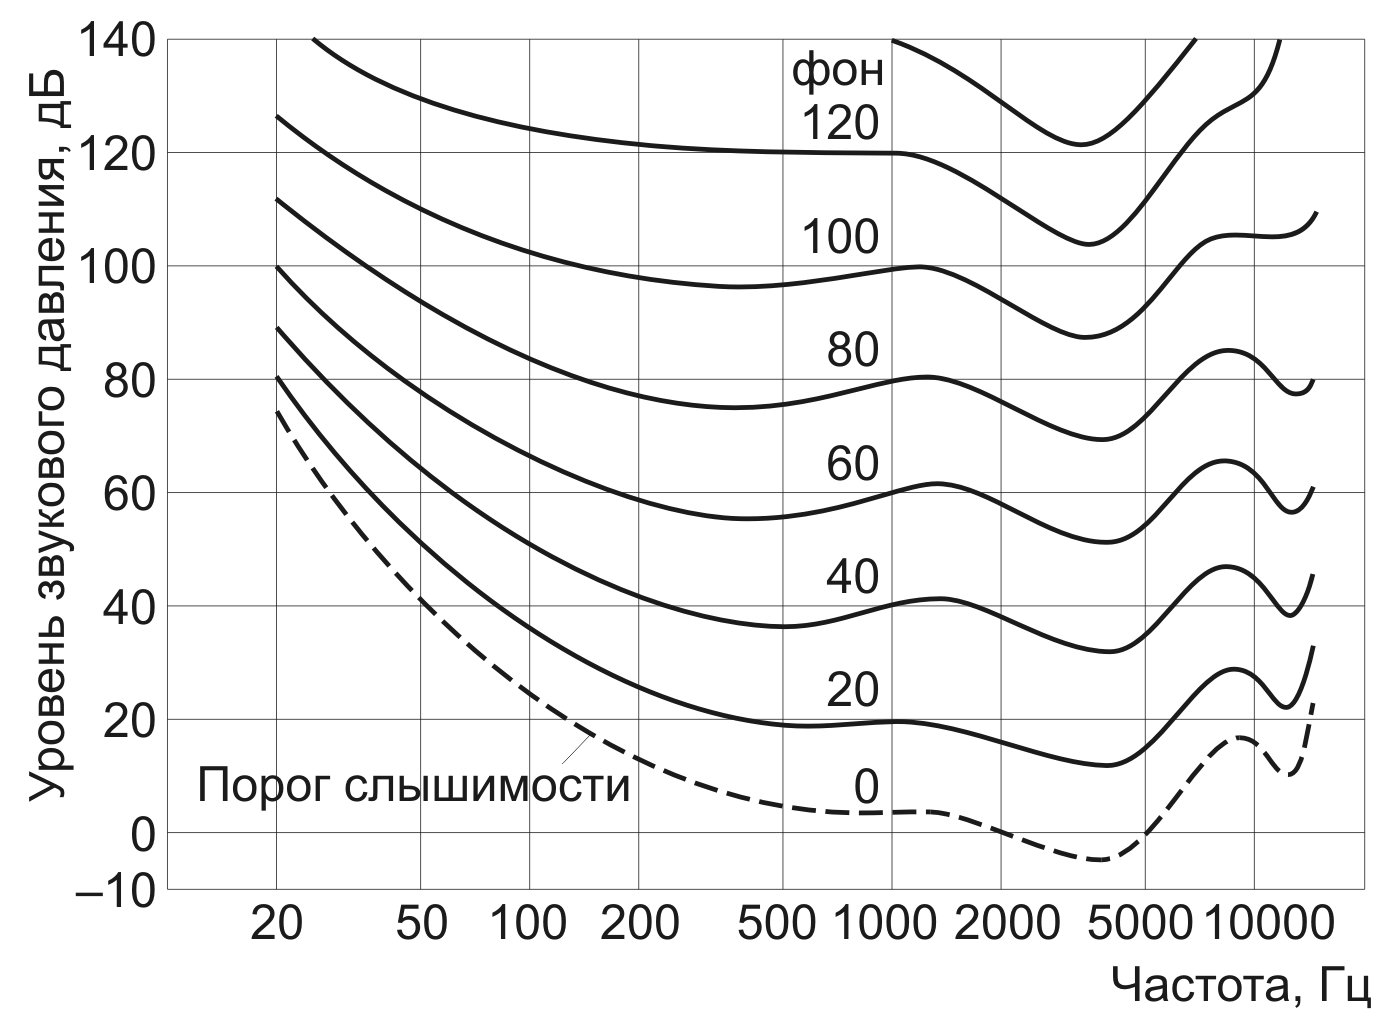
\includegraphics[scale=2.2]{Gromkost.png}
	\caption{Контур равных громкостей}
	\label{sec:analysus:sound_contur}
\end{figure}

\begin{figure}[h]
\centering
	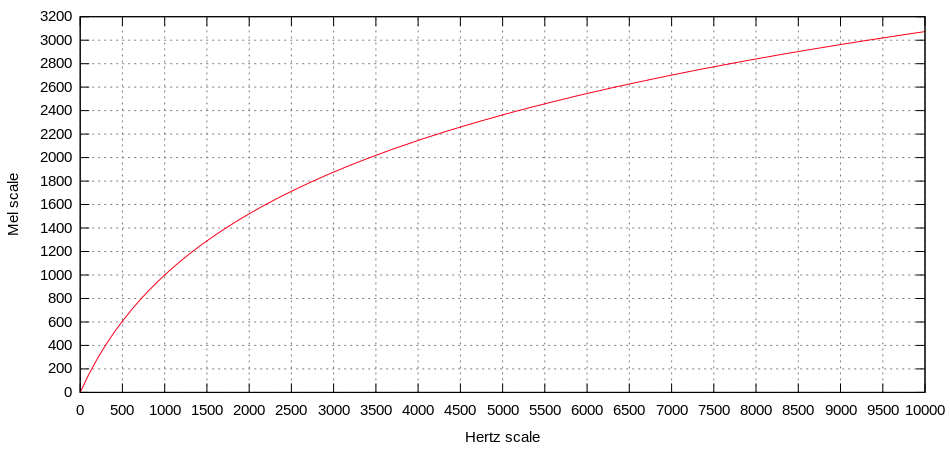
\includegraphics[scale=0.4]{mel-hz.png}
	\caption{Мел шкала}
	\label{sec:analysus:mel}
\end{figure}

До недавнего времени большинство методов машинного обучения и обработки сигналов использовались неструктурированными архитектурами. Эти архитектуры обычно содержат не более одного или двух слоев нелинейных функций. Примерами неглубоких архитектур являются модели гауссовых смесей, линейные или нелинейные динамические системы, условные случайные поля, модели максимальной энтропии, метод опорного вектора, логистическая регрессия, регрессия ядра, многослойные персептроны с одним скрытым слоем и экстремальными обучающими машинами. Например, метод опорного вектора используют модель разграничения линейных шаблонов с одним или нулевым уровнем преобразования объектов, когда используется трюк ядра или иным образом. Мелкие архитектуры были эффективны при решении многих простых или хорошо ограниченных проблем, но их ограниченное моделирование и репрезентативная власть могут создавать трудности при работе с более сложными приложениями реального мира, включающими естественные сигналы, такие как человеческая речь, естественный звук и язык, а также естественные изображения и визуальные сцены.

Однако механизмы восприятия информации человека (например, зрение и слух) указывают на необходимость глубоких архитектур для извлечения сложной структуры и создания внутреннего представления. Например, системы производства и восприятия речи человека оснащены четко стратифицированными иерархическими структурами для преобразования информации с уровня сигнала на лингвистический уровень. В аналогичном ключе человеческое зрение также является иерархической по своей природе на уровне восприятия. Естественно полагать, что современное окружение может быть усовершенствовано при обработке этих типов естественных сигналов, если могут быть разработаны эффективные алгоритмы глубокого обучения.

Исторически сложилось так, что понятие глубокого обучения было основано на исследованиях искусственной нейронной сети. Нейронные сети с обратной связью со многими скрытыми слоями, которые часто называют глубокими нейронными сетями, являются хорошими примерами моделей С глубокой архитектурой. Обратное распространение, популяризированное в 1980-х годах, было широко известным алгоритмом для изучения параметров этих сетей. К сожалению, обратное распространение само по себе не очень хорошо работает для для обучения сетей с большим количеством скрытых слоев. Широкое присутствие локальных оптимумов в невыпуклой целевой функции глубоких сетей является основным источником трудностей в обучении. обратное распространение основано на локальном градиентном спуске и обычно начинается в некоторых случайных начальных точках. Обратное распространение, которое не используется в связке с чем-то, обычно попадает в ловушку в локальных оптимумах, и степень ошибки значительно возрастает по мере увеличения глубины сетей. Эта трудность частично отвечает за провалы большинства исследований машинного обучения и обработки сигналов от нейронных сетей до неглубоких моделей с функциями выпуклых потерь, для которых глобальный оптимум может быть эффективно получен за счет меньшей мощности моделирования.

Проблема оптимизации, связанная с глубокими моделями, была эмпирически облегчена с использованием трех методов: большего количества скрытых единиц, улучшенных алгоритмов обучения и лучших методов инициализации параметров.

Использование скрытых слоев со многими нейронами в глубокой нейронной сети значительно улучшает мощность моделирования глубокой нейронной сети и создает много достаточно близких к оптимальным конфигураций. Даже если параметры обучения  захвачены в локальный оптимум, результат, получаемый глубокой нейронной сетью, может все же работать достаточно хорошо, так как вероятность плохого локального оптимума ниже, чем при использовании небольшого числа нейронов в сети. Однако использование глубоких и широких нейронных сетей потребовало бы огромной вычислительной мощности во время процесса обучения, и это одна из причин, почему только в последние годы исследователи начали серьезно изучать как глубокие, так и широкие нейронные сети.

Более эффективные алгоритмы обучения также способствовали успеху глубоких нейронных сетей. Например, стохастические алгоритмы обратного распространения вместо алгоритмов обратного распространения, оценивающих небольшие множества элементов, используемые для обучения глубоких нейронных сетей в настоящее время. Отчасти это связано с тем, что алгоритм стохастического градиента является наиболее эффективным алгоритмом, когда обучение осуществляется на одной машине, а обучающий набор является большим. Но, что более важно, алгоритм стохастичего градиентного спуска часто может выпрыгивать из локального оптимума из-за шумных градиентов, оцененных из одной или нескольких партий выборок. Аналогичные способности продемонстрировали другие алгоритмы обучения, такие как методы подпространства Крылова.

Для проблемы с обчень большим количеством локальных оптимумов для глубокой нейронной сети очевидно, что лучшие методы инициализации параметров приведут к улучшению моделей, поскольку оптимизация начинается с этих исходных параметров. Однако до недавнего времени не было известно как эффективно инициализировать параметры глубокой нейронной сети.

Метод инициализации параметров глубокой нейронной сети, который привлек наибольшее внимание, - это метод без учителя. В этих работах был введен класс глубоких байесовских вероятностных генеративных моделей, называемых сетью глубоких убеждений. Для изучения параметров в сетей глубоких убеждений был разработан жадный алгоритм обучения. Поэтапно, обрабатывая каждую пару слоев в сети глубоких убеждений как ограниченную машину Больцмана. Это позволяет оптимизировать параметры сети глубоких убеждений с вычислительной сложностью, линейной по глубине сети. Позже выяснилось, что параметры сетей глубоких убеждений могут быть непосредственно использованы в качестве начальных параметров многослойного перцептрона или глубокой нейронной сети и приводят к лучшим результатам, чем те, которые случайным образом инициализируются после контролируемого обучения методом обратного распространения ошибки, когда набор тренировок мал. Таким образом, глубокие нейронные сети изучались с неконтролируемым предварительным обучением сети глубоких убеждений с последующей тонкой настройкой обратной передачи. В последнее время исследователи стали более осторожными в определении отличий между глубокими нейронными сетями и сетями глубоких убеждений.

Процедура предварительной обработки сетями глубоких убеждений не является единственной, которая позволяет эффективно инициализировать глубокие нейронные сети. Альтернативный неконтролируемый подход, который одинаково хорошо работает, заключается в том, чтобы каждый раз перестраивать глубокую нейронную сеть, рассматривая каждую пару уровней как де-шумирующий автокодер, регулируемый путем установки произвольного подмножества входных данных на ноль. Другой альтернативой является использование контрастных автоэнкодеров для одной и той же цели, предпочитая модели, которые менее чувствительны к входным вариациям, то есть наказывают градиент активности скрытых единиц по отношению к входам. Кроме того, была разработана разрешающая симметричная машина, которая имеет очень похожую архитектуру для ограниченной машины Больцмана как структурные блоки сетей глубоких убеждений. В принципе, разрешающая симментричная машина также может использоваться для эффективной инициализации параметров глубокой нейронной сети. Было показано, что помимо неконтролируемой предварительной подготовки, контролируемая предварительная обработка, или иногда называемая дискриминационная предварительная обработка, так же показала себя эффективным методом, а в случаях, когда размеченных данных достаточно, показывает себя лучше, чем неконтролируемые техники предварительной обработки. Идея дискриминирующей предварительной подготовки состоит в том, чтобы начать с модели с одним скрытым слоем, обученным с помощью метода обратного распространения ошибки. Каждый раз, когда мы хотим добавить новый скрытый слой, мы заменяем выходной слой случайным образом инициализированным новым скрытым и выходным слоями и тренируем весь новый многоуровневый перцептрон или глубокую нейронную сеть с использованием метода обратного распространения ошибки. В отличие от неконтролируемых методов предварительной обработки, для метода дискриминирующей предварительной обработки требуются размеченные данные.

Как описано выше, глубокое обучение относится к довольно широкому классу методов машинного обучения и архитектур, с отличием от использования многих уровней нелинейной обработки информации, которые являются иерархическими по своей природе. В зависимости от того, как архитектуры и методы предназначены для использования, например, синтез и генерация или распознавание и классификация, можно широко классифицировать большую часть работы в этой области на три класса:
\begin{enumerate}
	\item генерирующие глубокие архитектуры;
	\item дискриминационные глубокие архитектуры;
	\item гибридная глубокая архитектура.
\end{enumerate}

Генерирующие глубокие архитектуры предназначены для захвата корреляций наблюдаемых или видимых данных высокого порядка для анализа или синтеза шаблоан и характеризуют совместные статистические распределения видимых данных и связанных с ними классов. В последнем случае использование правила Байеса может превратить этот тип архитектуры в дискриминационный.

Дискриминационные глубокие архитектуры, которые призваны непосредственно обеспечивать дискриминационную силу для целей классификации шаблонов, часто характеризуя последующие распределения классов, обусловленные видимыми данными.

Гибридные глубокие архитектуры, где целью является дискриминация, которая помогает с результатами генерирующих архитектур посредством лучшей оптимизации и регуляризации, или где дискриминационные критерии используются для изучения параметров в любой из моделей с глубокой генерацией.

В соответствии с общепринятой традицией машинного обучения, может быть естественным классифицировать методы глубокого обучения на глубокие дискриминационные модели, такие как глубокие нейронные сети, и модели с глубокой вероятностной генерацией, такие как сети глубокого убеждения. Однако в этой схеме классификации отсутствует ключевая информация, полученная в ходе глубоких исследований по вопросу о том, как генеративные модели могут значительно улучшить подготовку глубоких нейронных сетей и других глубоких дискриминационных моделей посредством лучшей регуляризации. Кроме того, модели с глубокой генерацией необязательно должны быть вероятностными, например, глубоким автоенкодером, многокоординатным автоэнкодером. Тем не менее, традиционная двухсторонняя классификация действительно указывает на несколько ключевых различий между глубокими дискриминационными моделями и глубокими порождающими вероятностными моделями. По сравнению с этими двумя, глубокие дискриминационные модели, такие как глубокие нейронные сети, обычно более эффективны для обучения и тестирования, более гибкие для построения и более подходящие для сквозного обучения сложным системам. С другой стороны, глубокие вероятностные модели легче интерпретировать, проще встраивать знания домена, проще составлять и легче справляться с неопределенностью, но, как правило, трудноразрешимы для вывода и обучения для сложных систем.

Традиционная нейронная сеть использовалась для распознавания речи в течение многих лет. При использовании в одиночку её производительность обычно ниже, чем современные системы скрытых марковских моделей с вероятностями наблюдения, аппроксимированными гауссовскими моделью смеси. С тех пор, как несколько лет назад технология глубокого обучения была успешно применена к анализу звука и крупным задачам распознавания речи путем интеграции мощной дискриминирующей обучающей способности глубокой нейронной сети с возможностями последовательного моделирования скрытых марковских моделей.

В экспериментах раннего фонетического распознавания использовалась стандартная объектная функция на основе кадра в классификации статических характеристик, кросс-энтропия, для оптимизации весов глубокой нейронной сети. Параметры перехода и оценки языковой модели были получены из скрытой модели маркова и прошли обучение независимо от весов глубокой нейронной сети. Тем не менее, в течение долгой истории исследований скрытых моделей Маркова было известно, что критерии классификации последовательности могут быть очень полезными для повышения точности распознавания речи и распознавания. Это связано с тем, что критерии классификации последовательностей более непосредственно коррелируют с показателем эффективности, чем кросс-энтропия.

Преимущество использования таких классификационных критериев последовательности было показано на неглубоких нейронных сетях. Один популярный тип критерия классификации последовательностей, максимальная взаимная информация, был успешно применен для изучения весов глубокой нейронной сети для задачи распознавания голоса. Использование кросс-энтропии для обучения глубокой нейронной сети для распознавания последовательности абонентов явно не учитывает тот факт, что соседние кадры имеют меньшие расстояния между назначенными распределениями вероятности по меткам класса звонков. Чтобы преодолеть этот недостаток, можно оптимизировать условную вероятность всей последовательности меток, учитывая всю видимую характеристику высказывания или эквивалентную скрытую функциональную последовательность, выделенную глубокой нейронной сетью. Чтобы оптимизировать условную вероятность журнала на данных обучения, мы берем градиент над параметрами активации, параметрами перехода и весами нижнего слоя, а затем продолжаем обратное распространение ошибки, определенной на уровне предложения.

Далее была разработана сверточная структура, которая накладывается на ограниченную машину Больцмана при создании сети глубокого убеждения. Свертка выполняется во времени путем совместного использования весов между скрытыми единицами в попытке обнаружить одну и ту же инвариантную функцию в разные моменты времени. Затем выполняется операция максимального пула, где достигаются максимальные активации по малым временным окрестностям скрытых единиц, что доказывает некоторую локальную временную инвариантность. Полученная сверточная сеть глубокого убеждения применяется к аудио и речевым данным для ряда задач, включая распознавание музыки исполнителя и жанровую классификацию, идентификацию спикера, гендерную классификацию говорящего и классификацию звонка, с обнадеживающими результатами.

Понятие свертки во времени было создано в нейронных сетях временного смещения как мелкая нейронная сеть, разработанная на ранних этапах исследований задачи распознавании речи. Только недавно при использовании глубоких архитектур, было обнаружено, что частотное распределение веса более эффективно для высокопроизводительного распознавания звонков, чем во временной области, как в предыдущей технологии нейронных сетей временного смещения. Эти исследования также показывают, что проектирование пула в глубокой сверточной нейронной сети для правильного компромисса между инвариантностью к длине голосового тракта и дискриминацией между звуками речи приводит к еще лучшему распознаванию. Эти результаты также указывают на направление соотношения между дискриминацией траектории и инвариантностью, выраженной во всей динамической структуре речи, определенной в смешанных временных и частотных областях, с использованием свертки и объединения. Более того, самые последние исследования показывают, что сверточные нейронные сети также полезны для широкого распознавания речи на основе словаря и далее демонстрируют, что несколько сверточных слоев обеспечивают еще большее улучшение, когда сверточные слои используют большое количество ядер свертки или карт признаков.

В дополнение к ограниченной машине Больцмана, глубоким нейронным сетям, другие глубокие модели также были разработаны и опубликованы в литературе для обработки речи и связанных с ней приложений. Например, глубоко структурированное поле случайных состояний, которое содержит много уровней случайных состояний, успешно использовалось в задаче идентификации языка, распознавании звонков, последовательной разметки на естественном языке и доверительная калибровка в распознавании речи. Кроме того, в то время как рекуррентные нейронные сети дали успешные результаты в ранних исследованиях в распознавании звонков, было непросто повторять результаты из-за сложности в обучении, не говоря уже о расширении для более крупных задач распознавания речи. С тех пор алгоритмы обучения для рекуррентных нейронных сетей значительно улучшились, и в последнее время были получены гораздо лучшие результаты с использованием рекуррентных нейронных сетей. Рекуррентные нейронные сети также недавно были применены к приложениям для обработки музыки, где в RNN исследуется использование выпрямленных линейных скрытых единиц вместо логистической или тангенциальной нелинейности. Исправленные линейные единицы вычисляют максимум из ноля и значения и приводят к уменьшенным градиентам, меньшей диффузии в рекуррентных нейронных сетях и более быстрому обучению.
